\documentclass{article}
\usepackage[utf8]{inputenc}
\usepackage[spanish]{babel}
\usepackage{ragged2e}
\usepackage{graphicx}
\graphicspath{ {images/} }
\usepackage{url}


\begin{document}

\begin{titlepage}
    \begin{center}
        \vspace*{1cm}
        
        \Huge
        \textbf{Informe Parcial I}
            
        \vspace{0.5cm}
        \LARGE
       \textit{ Informática II}
            
        \vspace{1.5cm}
            
        \textbf{ESTEBAN JARAMILLO PÉREZ\\
        SANTIAGO MUÑOZ JIMÉNEZ\\
        DANIEL ALEJANDRO VALENCIA}
            
        \vfill
            
        \vspace{0.8cm}
            
        \Large
        Despartamento de Ingeniería Electrónica y Telecomunicaciones\\
        Universidad de Antioquia\\
        Medellín\\
        Febrero de 2022
            
    \end{center}
\end{titlepage}

\tableofcontents
\newpage
\newpage
\section{Introducción}
\label{Introducción}
Desde que se crea un sistema de información el cual ha hecho que la vida cotidiana se desarrolle con una mayor facilidad, hemos dependido de está llegando a ser un punto vital para el desarrollo de nuestras vidas, pero como en todo se puede ver que también hay riesgos, hay quienes vician este beneficio y lo convertirán en un método para vivir a costa de lo que otros hacen y por este medio resulta aún más peligroso ya que no solo tienes peligro de perder algo si no también está en juego tu integridad como persona.\\
\newline
En vista de dicho panorama se crean constantemente recursos con los cuales se pueda tener una defensa sólida y como tal son muchas las personas las que se dedican a estos medios digitales,
En la actualidad hay muchos sectores de la industria que manejan su información en medios electrónicos y por la gran cantidad de información sensible que manejan se ven obligados a protegerse contra robos informáticos, muchos son los métodos que se pueden llevar a cabo para protegerse, uno de los mas utilizados contra esto es el método de encriptación.\\
\newline
Esta vez estaremos trabajando para una de las zonas de la industria que es más sensible a este tipo de ataques y por tal requieren una mayor seguridad y estos son lo bancos, en este proyecto abordaremos este problema con un programa que hará la encriptación automáticamente y nos ayudará a darle una solución rápida para este dilema.

\newpage
\section{Resumen}
\label{Resumen}
En un mundo plagado de tecnologías que nos conecta a través de redes informáticas circula nuestra información personal y esta es susceptible a la a ser interceptada por terceras personas las cuales pueden utilizar dicha información para extorsiones o robo, por ellos se emplean diferentes técnicas para resolver dicha dificultad, de estas la encriptación de la información es una de las más útiles al poner caracteres erróneos haciendo no legible su contenido.\\
\newline
En este texto se le dará desarrollo a un proyecto cuyo uso se verá aplicado a la encriptación de información para la seguridad en la transmisión de esta, dicho proyecto se realizará de forma física con un Arduino y un circuito integrado y en forma digital desarrollado en la plataforma tinkercad y QT


\newpage
\section{Objetivos de la practica}
\label{objetivos}
\textbf{Objetivo general}\\
Desarrollar un sistema de comunicación entre máquinas que pasen la información obtenida del usuario utilizando las herramientas requeridas en clase, con la meta de realizar un dispositivo para un banco ficticio que pueda transmitir cierta información desde los computadores de oficina a un computador donde se recolecta la información, encriptarla y desencriptarla, siendo así una fuente de información fiable y segura.\\



\textbf{Objetivo Específicos}

\justifying
\begin{itemize}

    \item Utilizar el circuito integrado 74HC595 de forma independiente con pulsadores o switches desarrollando con éxito la transmisión de bits de forma paralela por medio físico acortando así las líneas de código a utilizar y por ende reduciendo el peso de nuestro programa.

    
    \item Desarrollar nuestro código haciendo uso de Qt para utilizar como recurso las ayudas que se tienen en dicho ambiente de trabajo, llegando a realizar un programa de encriptado completo.

    \item  Realizar la conexión 2 Arduino entre sí, utilizando la herramienta tinkercad y con nuestro código desarrollado pasado a lo que requiere un Arduino para su funcionamiento se logra hacer una comunicación de datos entre las placas en un solo sentido.


    \item Desarrollar una conexión en uno de los Arduino con una pantalla LCD y con el fin observar los resultados del proyecto mostrando la efectividad de este sistema para su implementación.

\end{itemize}

\newpage
\section{Marco Teórico}
\label{Marco Teórico}
Los delitos informáticos son todas las acciones delictivas o no autorizadas que se hacen mediante dispositivos electrónicos e internet, estos delitos empezaron antes de que el sistema jurídico comenzará a vislumbrar dicho escenario, por lo cual poco a poco se van haciendo más y más normas que ayuden a controlar estos delitos.\\
\newline
Los delitos pueden ser espionaje, fraudes, accesos no autorizados, robo de software y robo de servicio, en este caso se aborda desde el punto de vista del fraude y espionaje, para evitar los fraudes en un mundo viciado por el dinero que guía todas estas maldades.\\
\newline
El desarrollo de este documento se llevará a cabo con diferentes programas y medios físicos de los se hablará a continuación:\\

Arduino: Es una plataforma electrónica la cual es basada en hardware y software fácil de manejar y permite crear diferentes tipos de microordenadores y darles diferentes usos a estos, el Arduino cuenta con un circuito integrado en el cual se pueden grabar instrucción y se puede conectar a diferentes tipos de periféricos ya sea de entrada o salida.\\

Qt: aplicación multiplataforma que se utiliza para desarrollar software que se puede utilizar en diferentes hardware o sistemas operativos.\\

Tinkercad: tinkercad es un software de uso libre de diseñado y modelado 3d.\\

Con la ayuda de estos programas se desarrollara un software efectivo para la encriptación de información y así protegerla de toda persona ajena a esta información, a dicha solución se llegara a través de una encriptación de la información añadiendo información no válida y luego convirtiéndola a binario para que pueda ser transmitida.



\newpage
\section{Uso del circuito integrado 74HC595.}
\label{74HC595}


Es un Chip que permite el desplazamiento de bits en un registro, es decir, que permite el ingreso serial (un bit) de datos, para luego obtener una salida en paralelo (8 bits); dependeran de los valores de entrada en serie (3 bits) y de los que ya están almacenados.

Este sistema es conocido por su tipo de desplazamiento en serie-paralelo, que con una sola entrada se pueden controlar las ocho salidas.Este mecanismo es controlado por una señal de reloj, el cual es usado para llevar el ritmo al que trabajara.Un ejemplo claro de este dispositivo es en el uso control original de Nintendo que necesita presionar todos los botones en serie.(cada pulso de un botón, es transformado por el 595 en una salida de 8 bits).

La figura 1 presenta un proceso donde al ser aplicada una pulsación, sucede que cada bit se mueve una posición a la izquierda,por ejemplo, el bit 7 cambia al valor que estaba en el 6 y así sucesivamente.También al llevar a cabo la pulsación, el PIN DATA, llevará un registro de altos y bajos, donde el primero marcará 1’s y el segundo 0’s

Con respecto a la figura 1 el PIN “latch” es utilizado para realizar una copia del DATA(Shift Register), que cada vez que este va recibiendo información, manda esos 8 bits al latch (Storage Register), si la salida se encuentra habilitada, los bits del latch son activados en los pin de salida (Output).


\begin{center}
\includegraphics[scale=0.5]{figura1}
imagen tomada de: https://lastminuteengineers.com/

\end{center}
\newpage

A continuación se mostrará el paso a paso y la utilidad que se le dio a los siguientes ejemplos.\newline

\begin{justify}
\textbf{(1)Circuito 595 con pulsador:} \\
 Se empleo un arduino, unas luces led, unas resistencias, un pequeño pulsador para probar el uso del reloj , la tierra (cable negro) y el positivo (cable rojo) se pegaran a la placa, sin el uso de estos dos no hara un correcto funcionamiento, ademas el uso de las salidas (cables azules) son usados para poder encender los leds, la entrada (cable verde) y el reloj de registro de desplazamiento (cable naranja) se utilizaron unidos al arduino, esto es debido a que con el uso de un pulsador, el voltaje se sobrepasaba, aunque con el uso de la bateria de 9V no era sufieciente, esto hacia que el circuito se quemara. Por otro lado, el reloj de salida, el que permite el ritmo de trabajo, es utilizado por medio de este pulsador, en este es necesario el uso de dos resistencia para llevar el control del voltaje y también el uso de un cable positivo, cada vez que se le presiona, este envía la señal y de esta forma permite llevar la información, esta es simulada con los leds encendidos.
 \end{justify}

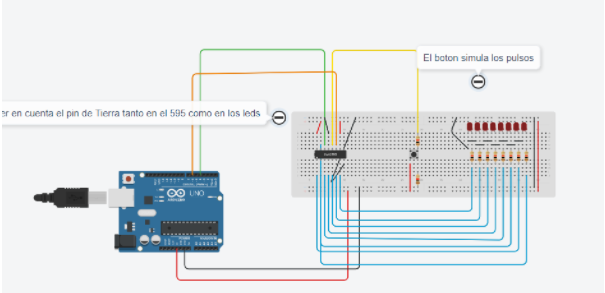
\includegraphics[scale=0.5]{figura2}
\centering
\textbf{Apoyado en el anexo 1}
\newline
\newline
\newline

\begin{justify}


\textbf{(1)Circuito 595 sin pulsador:}\\
Se empleó un arduino, unas luces led, unas resistencias y una placa. La tierra (cable negro) y el positivo (cable rojo) se pegaran a la placa, sin el uso de estos dos no hara un correcto funcionamiento, ademas el uso de las salidas (cables azules) son usados para poder encender los leds, la entrada (cable verde), el reloj de registro de desplazamiento (cable naranja) y el reloj de salida(cable amarillo).Como muestra la imagen cada uno esta conectado al arduino y al 595, permitiendo un correcto funcionamiento y el voltaje adecuado, es importante tener en cuenta el lugar al que va colocado cada cable, de lo contrario podrian ocurrir errores como lo son una mala ejecucion o el daño del circuito 595.
\end{justify}

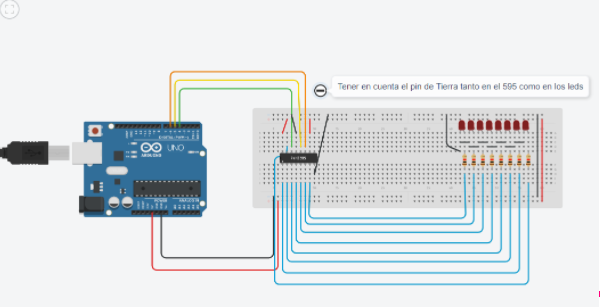
\includegraphics[scale=0.5]{figura3.png}
\centering
\textbf{Apoyado en el anexo 2}
\newline
\newline
\newline


\newpage
\section{Conexión entre dos Arduinos}
\label{Comunicación entre dos Arduinos}
\begin{justify}
El proceso que será usado consiste en conectar ambos arduinos definiendo a uno como Master o maestro y otro Slave o esclavo quien recibirá la información enviada por el primero, es por está razón que ambos tendrán codigos independientes.\\
\end{justify}
\begin{justify}

•	0: RX (pin por el que RECIBE los datos serie)\\
•	1: TX (pin por el que ENVÍA los datos serie)\\ 

\end{justify}
\begin{justify}

Un ejemplo de aplicación de la comunicación entre ambos arduinos puede ser:\\
Si envía una "r", el esclavo hará parpadear su led (d13) rápido.
Si envía una "l", el esclavo hará parpadear su led (d13) lento.\\
\end{justify}

\begin{justify}
Teniendo en cuenta que la información, en este caso caracter, será enviada desde el Master hasta el Slave cada tres segundos.
\end{justify}
\newpage
\centering Conexión entre arduinos I2C\\

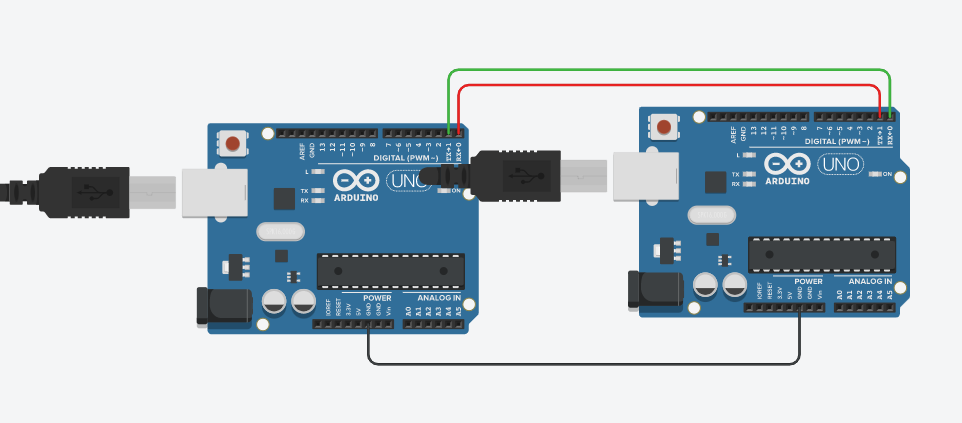
\includegraphics[scale=0.3]{figura4.png}\\

\textbf{Código ejemplo Arduino Master: }
\begin{verbatim}

void setup(){ 
  Serial.begin(9600);
}
void loop()
{ Serial.write("r");
  delay(3000);
  Serial.write("l");
  delay(3000);
}

\end{verbatim}

\textbf{Código ejemplo Arduino Slave: }
\begin{verbatim}

void setup(){ 
  pinMode(13,OUTPUT);
  Serial.begin(9600);
}
void loop(){ 
        char dato= Serial.read();//Guardamos en la variable dato el valor leido
        switch(dato){ //Comprobamos el dato
         case 'r':  //Si recibimos una 'r' ...
          for(int i=0; i<20; i++){
               digitalWrite(13,HIGH);
               delay(80);
               digitalWrite(13,LOW);
               delay(80);
          }
          break;
         case 'l':    //si recibimos una 'l' ...
         for(int i=0; i<10; i++){
               digitalWrite(13,HIGH);
               delay(1000);
               digitalWrite(13,LOW);
               delay(1000);
          }
          break;
          default:
           digitalWrite(13,LOW);
           break;
        }
}

\end{verbatim}

El reultado con el uso del LED sería el siguiente:

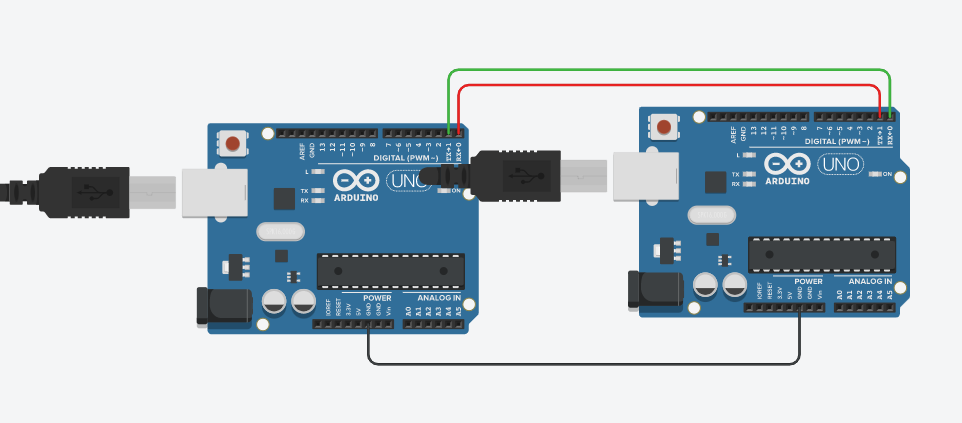
\includegraphics[scale=0.4]{figura4.png}
\newpage
\section{Bloque de desencriptación}
\label{Bloque de desencriptación}
\begin{justify}


Para el bloque de desencriptación, realizamos un panorama general en la aplicación Qt, con el fin de identificar el comportamiento del sistema correspondiente, en este caso, identificar la clave 69 y los códigos validos serán aquellos que se encuentren en la penúltima y antepenúltima posición, además que cinco posiciones antes deben aparecer un 18.
Con esta información, fue necesario evaluar las condiciones y como filtrar dicha información para encontrar los códigos válidos, de manera que fuera posible encontrar la clave, operar sobre ella y extraer los datos correspondientes, en el caso mostrándolos en pantalla.
\end{justify}
\begin{verbatim}
#include<iostream>
#include<sstream>
using namespace std;

string condicion(float vector[], int pos, string message);

int main() {
    int i;
    string message;
    int n;
    int vector[]={15,16,80,18,12,15,17,19,69,81};

    n = sizeof (vector);
    message = "";

    for (i=0;i<=n-1;i++) {
        if (vector[i]==18) {
            if (vector[i]==18 && vector[i+5]==69) {
                cout<<vector[i+2]<<endl;
                cout<<vector[i+3]<<endl;
            }
        }

    }
    
    return 0;
}


\end{verbatim}
\newpage
\centering Conexión entre arduinos usando puertos digitales\\
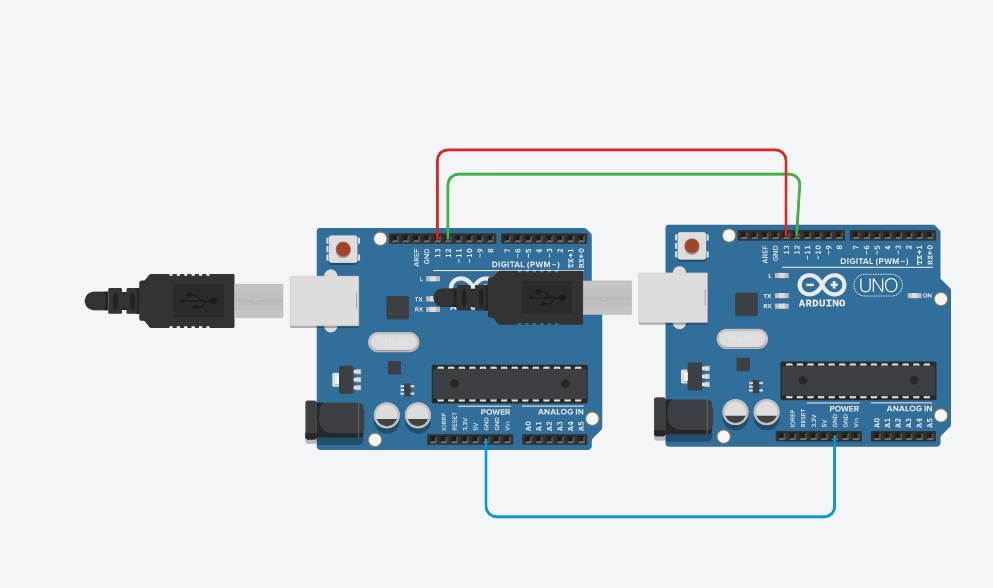
\includegraphics[scale=0.3]{figura6.png}\\
\begin{verbatim}
    int vector[] = {15,16,80,18,12,15,17,19,69,81};
void setup()
{
  pinMode(13, OUTPUT);
  pinMode(12, OUTPUT);
  Serial.begin(9600);
}

void loop()
{
  for(int i = 0; i < 10; i++){
    digitalWrite(12, HIGH);
    for(int j = 0; j < 8; j++){
    	digitalWrite(13,((vector[i] << j);
		delay(100);
    }
     digitalWrite(12,LOW);
  }
}

// conexion de arduinos con puertos digitales
// segundo arduino
int val[8];
void setup()
{
  pinMode(13, OUTPUT);
  pinMode(12, OUTPUT);
  Serial.begin(9600);
}

void loop()
{
  if(digitalRead(12)){
    for(int i = 0; i <8; i++){
   		val[i] = digitalRead(13);
      	Serial.print(val[i]);
      	delay(100);
    } 
    Serial.println();
  }
}
\end{verbatim}

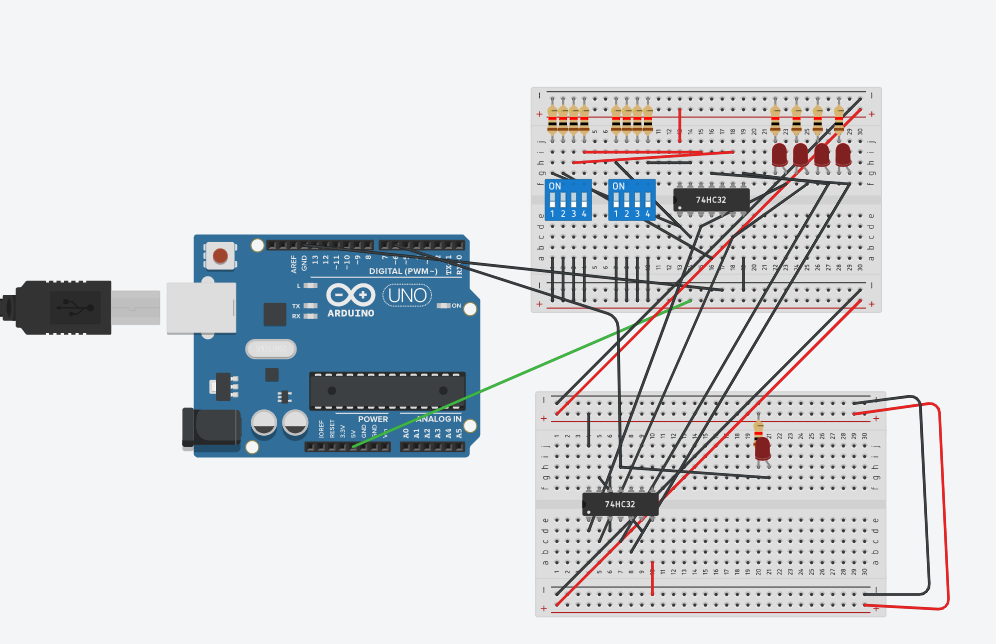
\includegraphics[scale=0.3]{figura7.png}\\
\begin{verbatim}
    //Pruebas desencriptar
int aux=0;
int key=9;
void setup()
{
  Serial.begin(9600);
  pinMode(6, INPUT);
}

void loop()
{
  
  int temp = digitalRead(6);
  if (temp!=key){
    aux=0;
  if(temp==18)
    if(aux==5)
    //almacenar clave
    else
  	Serial.println("Hay un 18");//5 psoiciones mas adelante hay un 69 hay clave
    aux=aux+1;
  key=temp;
    
  }
}
\end{verbatim}
\newpage
\section{Conclusiones}
\label{Conclusiones}
\begin{justify}
En un mundo que es dominado por medios informáticos y cada vez avanza hacia un futuro donde todo sea manejado por medio de lo digital también se vera un crecimiento en el riesgo de crímenes informáticos paralelo a este, como tal es deber de quienes tienen el conocimiento requerido para el manejo de estas redes de información el buscar diversas formas con las cuales se pueda proteger a la comunidad de estos elevados riesgos.\\

Con la construcción de este proyecto se a dado una pequeña ayuda a la lucha que se esta dando día a día, al encriptar nuestra información se eleva la dificultad para aquellos ajenos a esta, es como si tuviéramos una caja fuerte que resguarde nuestros secretos y el código de encriptación fuera la llave, si no se conoce este código se tendrá una dificultad elevada para tener acceso a esos recursos informáticos y así podemos prevenir crímenes informáticos como espionaje o fraude.
\end{justify}


\newpage
\section{Anexos}
\label{Anexos}
\begin{justify}


\textbf{(1)}
\url{https://www.tinkercad.com/things/6ROBFOLGDwK-copy-of-74hc595/editel?sharecode=t7hqpOIFHnGtsxOCjGsjoC3OBudnwDUmjirfRQvRiZU}
\newline
\newline
\textbf{(2-3)}
\url{https://www.tinkercad.com/things/6VynWWL64fP-74hc595/editel?sharecode=ot5gC80GJt7dIHeJV_Vv7UX7wF0xgc8KLDBU_-QefwY}
\newline
\newline
\textbf{(4)}
\url{https://www.instructables.com/I2C-between-Arduinos/}
\end{justify}
\newpage
\section{Referencias}
\label{Referencias}

\justify
Last Minute Engineers -. (2021). Last Minute Engineers. https://lastminuteengineers.com/\\
\newline
I. (2019, 18 julio). 74hc595: todo sobre el CI de registro de desplazamiento. Hardware libre. https://www.hwlibre.com/\\
\newline
S. (2019b, abril 24). Significado de Delitos informáticos. Significados. https://www.significados.com/delitos-informaticos/\\
\newline
Fernández, Y. (2020, 3 agosto). Qué es Arduino, cómo funciona y qué puedes hacer con uno. Xataka. https://www.xataka.com/basics/que-arduino-como-funciona-que-puedes-hacer-uno\\
\newline
¿Que es qt? - definicion de techopedia - Desarrollo - 2022. (2022). Icy Science. https://es.theastrologypage.com/qt\\

\url{4.2.1 M2: dos Arduinos · GitBook. (2022). Conectar dos Arduinos. https://catedu.github.io/programa-arduino-mediante-codigo/montaje_2_conectar_dos_arduinos.html}




\end{document}



